\documentclass{amsart}
\usepackage{amsfonts} % For math fonts
\usepackage{amsmath, amssymb, amsthm}
\usepackage{float}
\usepackage{enumitem}
\usepackage{graphicx}
\setlist[enumerate,1]{label=\arabic*.}
\setlist[enumerate,2]{label=\alph*.,itemindent=2em}
\setlist{topsep=0pt, leftmargin=*, labelsep=1em}


\usepackage{listings}
\usepackage{xcolor}

\lstset{
    language=Python,
    backgroundcolor=\color{black}, % Light gray background
    basicstyle=\ttfamily\small\color{white}, % Code style
    keywordstyle=\color{cyan}\bfseries, % Keywords style
    stringstyle=\color{yellow}, % Strings style
    commentstyle=\color{gray}, % Comments style
    frame=single, % Box around code
    rulecolor=\color{white}, % Frame color
    numbers=left, % Line numbers
    numberstyle=\tiny\color{white}, % Line number style
    breaklines=true, % Automatic line breaking
    showstringspaces=false
}


\title{HW 4 - 151A}
\author{Asher Christian 006-150-286}
\date{ 12.02.25}

\begin{document}
    \maketitle
    \section{Exercise 1}
    \begin{enumerate}[label = (\alph*)]
        \item $f(x) = \sin(2\pi x)$ $[a,b] = [0,1]$. \emph{ construct piecewise lienar polynomial
            that interpolates $f$ at $\{0,\frac{1}{2},1\}$ call it $P_{1,2}$.}\\
            \[
            S_0(0) = b_0 = 0 \;\; S_0(\frac{1}{2}) = \frac{1}{2}a_0 + b_0 = \frac{1}{2}a_0 = 0 \implies a_0 = 0
            .\] 
            \[
            S_1(\frac{1}{2}) = \frac{1}{2}a_1 + b_1 = 0 \;\; S_1(1) = a_1 + b_1 = 0 \implies a_1=b_1=0
            .\] 
            thus
            \[
                P_{1,2} = 0
            .\] 
        \item \emph{Repeat at $\{0,\frac{1}{4},\frac{1}{2},\frac{3}{4},1\}l$ and call it $P_{1,4}$}
             \[
            S_0(0) = b_0 = 0 \; S_0(\frac{1}{4}) = \frac{1}{4}a_0 = 1 \implies b_0 = 0 \;\; a_0 = 4\\
            .\] 
            \[
            S_1(\frac{1}{4}) = \frac{1}{4}a_1 + b_1 = 1 \;\; S_1(\frac{1}{2}) = \frac{1}{2}a_1 + b_1 = 0 \implies a_1 = -4 \;\; b_1 =2
            .\] 
            \[
            S_2(\frac{1}{2}) = \frac{1}{2}a_2 + b_2 = 0 \; S_2(\frac{3}{4}) = \frac{3}{4}a_2 + b_2 = -1 \implies a_2 = -4 \; b_2 = 2
            .\] 
            \[
            S_3(\frac{3}{4}) = \frac{3}{4}a_3 + b_3 = -1 \; S_3(1) = a_3 + b_3 = 0 \implies a_3 = 4 \; b_3 = 4
            .\] 
            \[
                P_{1,4} =
                \begin{cases}
                    4x & 0 \le x < \frac{1}{4}\\
                    -4x + 2 & \frac{1}{4} \le x < \frac{3}{4}\\
                    4x -4 & \frac{3}{4} \le x < 1\\
                \end{cases}
            .\] 
        \item Draw a graph
            \begin{figure}[h]
                \centering
                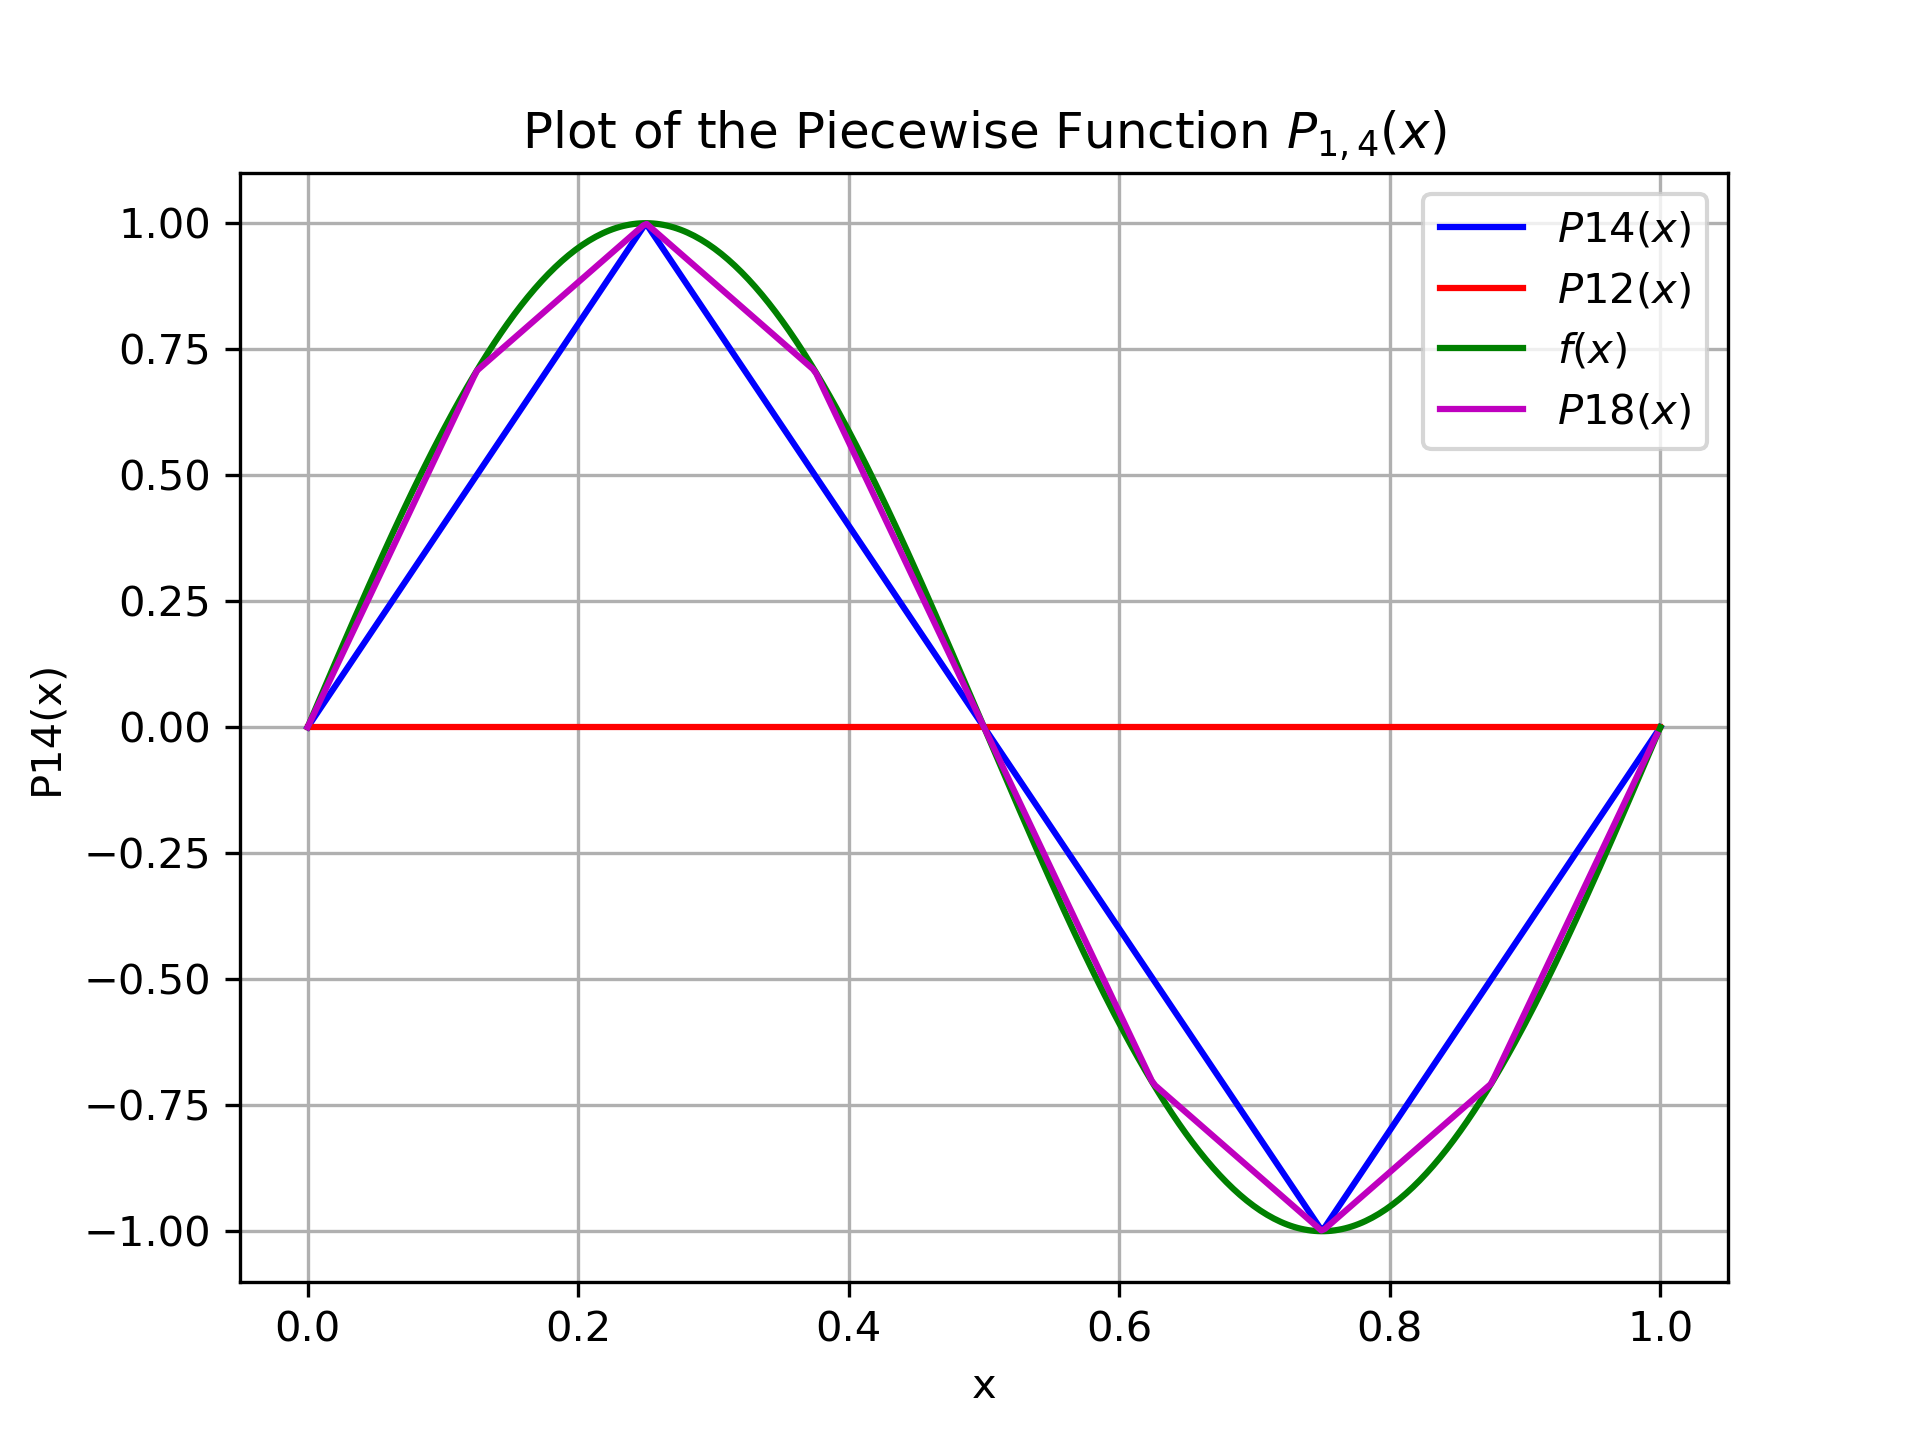
\includegraphics[width=0.8\textwidth]{plot.png}
                \caption{Plot of all functions}
                \label{fig:multiple_function}
            \end{figure}
            From this example we can intuitively conclude that the error $\lim_{n\to \infty}||f(x) - P_{1,n}(x)||_{L^{\infty}} = 0$
            \clearpage
        
    \end{enumerate}
    \section{Exercise 2}
    \emph{
        Let $f(x) = sin(\pi x)$ for $x \in [-1,1]$ and let $n \ge 1$ be an integer. Find points $x_0,...,x_n \in [-1,1]$ such
        that the polynomial interpolant $P_n$ of $f$ for these points satisfies the error estimate
        \[
            ||f - p_n||_{L^{\infty}([-1,1])} \le \frac{2}{(n+1)!}(\frac{\pi}{2})^{n+1}
        .\] 
    }
    Pick the Chebyshev nodes
    \[
    x_i = \cos(\frac{2 i+1}{2n+2}\pi)
    .\] 
    such that
    \[
        \prod_{k=0}^{n}(x-x_k) \le 2^{-n}
    .\] 
    on $[-1,1]$
    and note that
    \[
        |f^{n+1}(x)| \le \pi^{{n+1}}
    .\] 
    by application of chain rule for all $x$. additionally
    \begin{align*}
        |p_n(x)-f(x)| &= |\frac{f^{(n+1)}( \xi(x))}{(n+1)!}||\prod_{i=1}^{n}(x-x_i)|\\
                      &\le |\frac{\pi^{n+1}}{(n+1)!}2^{-n}|\\
                      &= \frac{2}{(n+1)!}(\frac{\pi}{2})^{n+1}
    \end{align*}
    on $[-1,1]$
    \section{Exercise 3}
    \[
    P_0(x)= 4.38125\left(x-0.1\right)^{3}-2.7512863\left(x-0.1\right)-0.29
    .\] 
    \[
    P_1(x) = -4.38125\left(x-0.2\right)^{3}+1.314375\left(x-0.2\right)^{2}-2.6198488\left(x-0.2\right)-0.56079734
    .\] 
    \[
    S(0.18) = -0.507859704 \;\; f(0.18) = -0.508123464354 \;\; |\frac{S(0.18) - f(0.18)}{f(0.18}| = 0.000519087135644
    .\] 
    \[
    S'(0.18) = -2.6671663 \;\; f'(0.18) = -2.65161682878 \;\; |\frac{S'(0.18)-f'(0.18)}{f'(0.18}| = 0.00586414713317
    .\] 
    \[
    S'(0.2) = -2.6198488 \;\; f'(0.2) = -2.6159201421 \\ |\frac{S'(0.2)-f'(0.2)}{f'(0.2)}| = 0.00150182639044
    .\] 
    They are similar but they are not the same.

    \section{Exercise 4}
    First
    \[
    f'(0.2) = -2.6159201421 
    .\] 
    For forward difference
    \[
    f'(x_0) \approx \frac{f(x_0+h)-f(x_0)}{h}  \implies f'(0.2) \approx \frac{-0.81401972 - (-0.56079734)}{0.1} = -2.53222379092  = p_0
    .\] 
    \[
    |\frac{p_0-f'(0.2)}{f'(0.2)}| = 0.0319949947344
    .\] 
    For central difference
    \[
    f'(x_0) \approx \frac{f(x_0+h)-f(x_0-h)}{2h} = \frac{-0.814019715979 - (-0.290049958347)}{.2} = -2.61984878816 = p_1
    .\] 
    \[
    |\frac{p_0-f'(0.2)}{f'(0.2)}| = 0.00150182186331
    .\] 

    \section{Exercise 5}
    \emph{
        \[
        f(x) = \frac{1}{1+25x^2}
        .\]  
        on the interval $[-1,1]$ with $N \in \{7, 11, 20\}$ nodes. do the following:
        \begin{enumerate}
            \item Lagrange Polynomial with $N$ equi-spaced nodes, $x_0 = -1, x_N = 1, h = \frac{2}{N-1}$ 
            \item Langrance polynomial with $N$ Chebyshev nodes, $x_k = \cos(\frac{2k+1}{2N}\pi)$
            \item Cubic spline interpolation with equi-spaced nodes and clamped boundary condition $S(x_0) = f'(x_0), \; S(x_N) = f'(x_N)$
        \end{enumerate}
    }
    \begin{figure}[h]
        \centering
        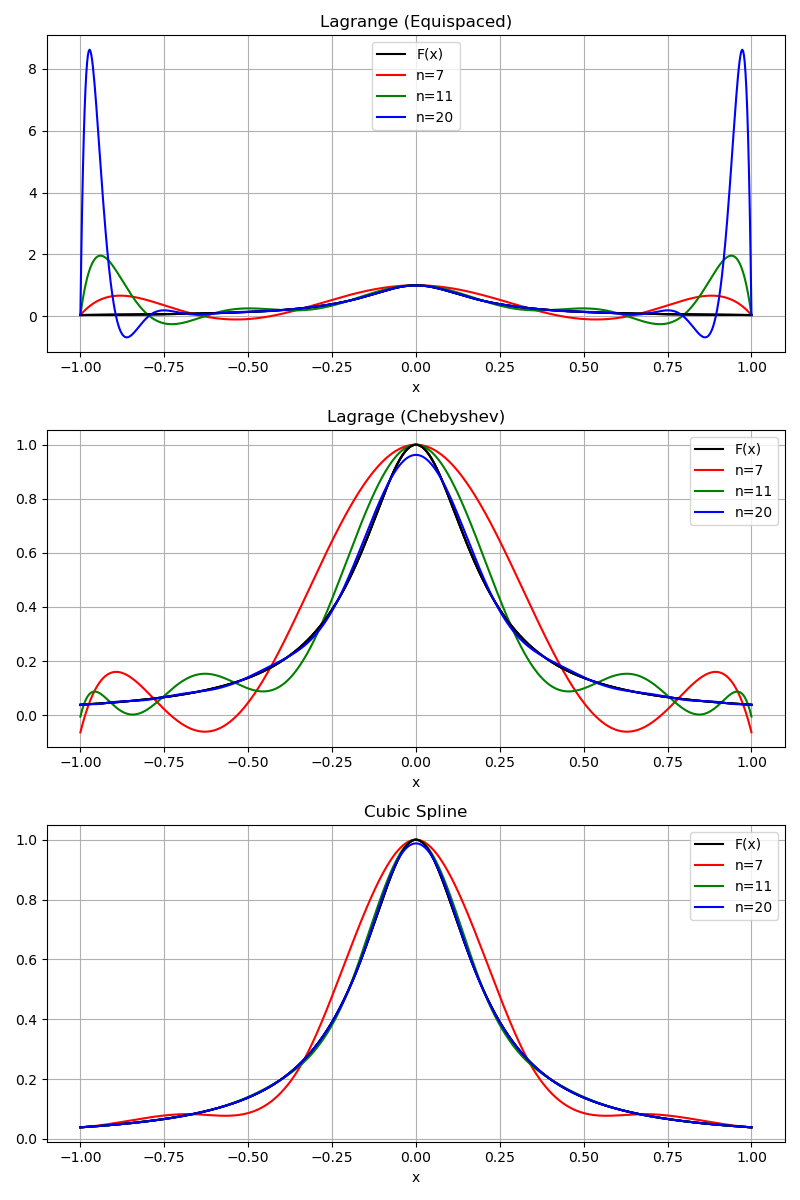
\includegraphics[width=0.8\textwidth]{multi-interpolant.png}
        \caption{Plot of all interpolations}
        \label{fig:multiple_function}
    \end{figure}
    \clearpage
    \begin{lstlisting}
    import numpy as np
    from scipy.interpolate import CubicSpline
    from scipy.interpolate import lagrange
    import matplotlib.pyplot as plt

    def f(x):
        return 1 / (1 + 25 * x**2)


    x_vals = np.linspace(-1,1,800)
    y_vals_f = f(x_vals)

    n_values = [7,11,20] # interpolation points

    fig, axs = plt.subplots(3,1,figsize=(8,12))
    titles = ["Lagrange (Equispaced)", "Lagrage (Chebyshev)", "Cubic Spline"]
    colors = ["r","g","b"]


    for i,n in enumerate(n_values):
        #Equispaced points
        x_equi_space = np.linspace(-1,1,n)
        y_equi_space = f(x_equi_space)

        #Lagrange with equispaced points
        lagrange_equi = lagrange(x_equi_space,y_equi_space)
        y_lagrange_equi = lagrange_equi(x_vals)

        # Lagrange with Chebyshev nodes
        x_cheby = np.cos([((2*k+1)/(2*n))*np.pi for k in range(0,n)])
        y_cheby = f(x_cheby)
        lagrange_cheby = lagrange(x_cheby,y_cheby)
        y_lagrange_cheby = lagrange_cheby(x_vals)

        #cubic Spline with equispaced points
        cubic_equi = CubicSpline(x_equi_space,y_equi_space, bc_type = ((1, 0.0739644970414),(1,-0.0739644970414)))
        y_cubic = cubic_equi(x_vals)

        #Plot for each interpolation method
        axs[0].plot(x_vals, y_vals_f, 'k', label="F(x)" if i == 0 else "")
        axs[0].plot(x_vals, y_lagrange_equi, color=colors[i], label=f"n={n}")

        axs[1].plot(x_vals, y_vals_f, 'k', label="F(x)" if i == 0 else "")
        axs[1].plot(x_vals, y_lagrange_cheby, color=colors[i], label=f"n={n}")

        axs[2].plot(x_vals, y_vals_f, 'k', label="F(x)" if i == 0 else "")
        axs[2].plot(x_vals, y_cubic, color=colors[i], label=f"n={n}")

    for i, ax in enumerate(axs):
        ax.set_title(titles[i])
        ax.set_xlabel("x")
        ax.grid(True)
        ax.legend()

    plt.tight_layout()

    plt.savefig("multi-interpolant.png")

    plt.show()
    \end{lstlisting}
    By observation, the equispaced lagrange polynomial suffers from Runge phenomena and is not an accurate interpolant.
    The chebyshev polynomai does not experience Runge Pheomena but still differs noticably from the original function even at 20 points.
    similarly by observation, cubic spline converges the fastest.

\end{document}
